\documentclass[12pt,oneside,brudnopis]{xelatex-mgr/xmgr}

\usepackage{amsmath}
\usepackage{blindtext}

\defaultfontfeatures{Scale=MatchLowercase}
\setmainfont[Numbers=OldStyle,Mapping=tex-text]{Minion Pro}
\setsansfont[Numbers=OldStyle,Mapping=tex-text]{Myriad Pro}
\setmonofont[Scale=0.75]{Monaco}

\wersja{wersja wstępna [\ymdtoday]}

\author{Bartłomiej Kruczyk}
\nralbumu{213603}
\email{bartlomiej.kruczyk@gmail.com}

\title{Efektywne algorytmy dla wielokątów wypukłych}
\date{2014}
\miejsce{Gdańsk}

\opiekun{dr Paweł Żyliński}

\newtheorem{problem}{Problem}

\includeonly{
  podstawowe_pojecia,
  lokalizacja_punktu,
  wyznaczanie_srednicy
}

\begin{document}

\begin{abstract}
  \blindtext[1]
\end{abstract}

\keywords{}

\maketitle

%%% Local Variables:
%%% mode: latex
%%% TeX-master: "masterthesis"
%%% TeX-engine: xetex
%%% End:

%% rozwinąć
\introduction{
  Przedstawione w niniejszej pracy problemy są wspólne dla
  wszystkich wielokątów, co pozwala na porównanie rozwiązań i ich
  efektywności dla wielokątów prostych i wypukłych. Przy każdym z nich
  zostanie przedstawiony problem uogólniony dla wielokątów prostych,
  następnie rozwiązanie dla wielokąta wypukłego wraz z analizą
  złożoności oraz poprawności algorytmu.
}

%%% Local Variables:
%%% mode: latex
%%% TeX-master: "masterthesis"
%%% TeX-engine: xetex
%%% End:

\chapter{Podstawowe pojęcia}\label{chap:pojecia}
W tym rozdziale zostaną przybliżone podstawowe pojęcia związane
z geometrią obliczeniową i problemami dotyczącymi wielokątów
wypukłych.

\begin{definicja}
  \emph{Wielokątem prostym} nazywamy taki wielokąt, że jedyne punkty
  płaszczyzny należące jednocześnie do dwóch jego krawędzi są jego
  wierzchołkami.
\end{definicja}

\begin{definicja}
  \emph{Wielokątem wypukłym} nazywamy wielokąt prosty którego wnętrze
  jest \emph{zbiorem wypukłym}, tzn.\ wszystkie punkty należące do
  odcinka łączącego dwa dowolne punkty ze zbioru należą do tego
  zbioru.
\end{definicja}

% brzeg wielokąta, wnętrze i zewnętrze wielokąta
% rysunki !

\begin{figure}[htb]
  \centering
  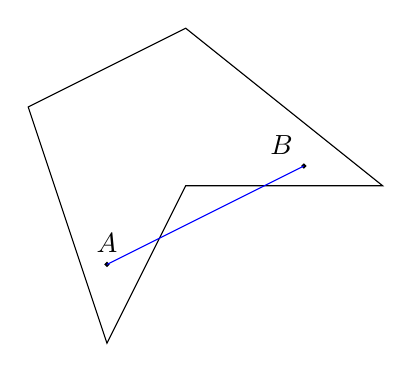
\begin{tikzpicture}
      \coordinate (p0) at (4.5,2);
      \coordinate (p1) at (2,4);
      \coordinate (p2) at (0,3);
      \coordinate (p4) at (1,0);
      \coordinate (p5) at (2,2);

      \draw (p0) -- (p1) -- (p2) -- (p4) -- (p5) -- cycle;

      \coordinate (a) at (1,1);
      \node [anchor=center,circle,draw,fill,inner sep=0.5pt,
        label={above:$A$}] at (a) {};

      \coordinate (b) at (3.5,2.25);
      \node [anchor=center,circle,draw,fill,inner sep=0.5pt,
        label={120:$B$}] at (b) {};

        \draw[blue] (a) -- (b);
  \end{tikzpicture}
  \caption{Przykład pięciokąta, który nie jest wypukły.}
\end{figure}

\begin{definicja}
  \emph{Średnicą zbioru punktów} nazywamy największą odległość
  pomiędzy dwoma punktami należącymi do tego zbioru.
\end{definicja}

\begin{definicja}
  Niech $p_{1}=(x_{1},y_{1})$, $p_{2}=(x_{2},y_{2})$,
  $p_{3}=(x_{3},y_{3})$ będą punktami na płaszczyźnie
  $\mathbb{R}^2$. \emph{Wyznacznikiem} współrzędnych tych punktów
  nazywamy liczbę

  \begin{center}
    \begin{math}
      X(p_1, p_2, p_3) =
      \begin{vmatrix}
        x_1 & y_1 & 1 \\
        x_2 & y_2 & 1 \\
        x_3 & y_3 & 1
      \end{vmatrix}
      .
    \end{math}
  \end{center}

  Kąt $\angle p_{1}p_{2}p_{3}$ nazywamy \emph{lewoskrętnym}, jeżeli
  wyznacznik $X(p_1, p_2, p_3)$ jest dodatni, w przeciwnym przypadku
  mówimy, że kąt ten jest \emph{prawoskrętny}.
\end{definicja}

\begin{definicja}
  \emph{Prostymi wspierającymi} dla wielokąta nazywamy takie proste,
  które przechodząc przez wierzchołek wielkąta nie przecinają jego
  wnętrza.
\end{definicja}

\begin{definicja}
  Mówimy, że para wierzchołków tworzy \emph{punkty antypodyczne},
  jeżeli można poprowadzić przez te wierzchołki przynajmniej dwie
  różne równoległe proste wspierające.
\end{definicja}

\begin{definicja}\label{def:bigo}
  Mówimy, że funkcja $f\colon \mathbb{N} \to \mathbb{R}$ jest co
  najwyżej rzędu $g$ (jest \emph{ograniczona} przez funkcję $g\colon
  \mathbb{N} \to \mathbb{R}$), gdy istnieją takie stałe $n_0 > 0$ oraz
  $c > 0$, że

  \begin{center}
    $\forall n \geq n_0\ f(n) \leq c \cdot g(n)$.
  \end{center}
\end{definicja}

W niniejszej pracy do opisu wydajności algorytmów będziemy korzystać z
\emph{notacji wielkiego O}. Jest to notacja asymptotycznego tempa
wzrostu wartości funkcji względem jej argumentów, w algorytmice
stosowana do charakterystyki złożoności obliczeniowej algorytmów
opisując ilość potrzebnych zasobów (czasu lub pamięci) w stosunku do
rozmiaru danych wejściowych. Zgodnie z tą notacją złożoność czasową
algorytmu o czasie działania $T(n) = f(n)$, gdzie $f(n)$ spełnia
definicję~\ref{def:bigo}, zapisalibyśmy jako $T(n) = O(g(n))$.

\begin{table}[htb]
  \centering

  \begin{tabular}{ll}
    \toprule
    $O(1)$ & stała \\
    \midrule
    $O(\log n)$ & logarytmiczna \\
    \midrule
    $O(n)$ & liniowa \\
    \midrule
    $O(n \log n)$ & liniowo-logarytmiczna \\
    \midrule
    $O(n^2)$ & kwadratowa \\
    \midrule
    $O(n^c)$ & wielomianowa \\
    \midrule
    $O(c^n)$ & wykładnicza $(c > 1)$ \\
    \midrule
    $O(n!)$ & ograniczona przez silnię \\
    \bottomrule
  \end{tabular}

  \caption{Najczęściej wyróżniane rzędy złożoności obliczeniowej,
    podane według rosnącej złożoności.}
\end{table}

W tej pracy \emph{efektywnym} algorytmem dla wielokąta wypukłego
będziemy nazywać algorytm o mniejszej złożoności obliczeniowej niż
najlepszy znany algorytm dla wielokąta prostego dla tego samego
problemu.

% przyjęte oznaczenia

%%% Local Variables:
%%% mode: latex
%%% TeX-master: "masterthesis"
%%% TeX-engine: xetex
%%% End:

\newcommand{\convexA}{
  \coordinate (p0) at (4.5,2);
  \coordinate (p1) at (4,3.25);
  \coordinate (p2) at (2,4);
  \coordinate (p3) at (1,3.5);
  \coordinate (p4) at (0,2);
  \coordinate (p5) at (2,0);
  \coordinate (p6) at (3.75,1);

  \draw (p0) -- (p1) -- (p2) -- (p3) -- (p4) -- (p5) -- (p6) -- cycle;
}

\newcommand{\convexB}{
  \coordinate (p0) at (3.5,     4);
  \coordinate (p1) at (1.5,     4.5);
  \coordinate (p2) at (0,       3.5);
  \coordinate (p3) at (-0.5,    1.5);
  \coordinate (p4) at (1.75,    0);
  \coordinate (p5) at (4,       1);

  \draw (p0) -- (p1) -- (p2) -- (p3) -- (p4) -- (p5) -- cycle;
}

\chapter{Lokalizacja punktu}
Problem lokalizacji punktu sformułowany jest następująco.

\begin{problem}[Lokalizacja punktu]
  Jeśli dany jest wielokąt prosty $P$ i punkt $z$ na płaszczyźnie,
  sprawdzić czy punkt $z$ należy do wnętrza $P$.
\end{problem}

Problem ten można rozwiązać w czasie $O(n)$ bez przetwarzania
wstępnego. Rozważmy poziomą prostą $l$ przechodząca przez punkt
$z$. Musimy rozważyć kilka przypadków.

\begin{itemize}
\item Jeśli $l$ nie przecina $P$, to $z$ leży na zewnątrz wielokąta.
  \begin{figure}[htp]
    \centering
    \begin{tikzpicture}
      \convexA

      \node [anchor=center,circle,draw,fill,inner sep=0.5pt,
      label={right:$p_0$}] at (p0) {};

      \node [anchor=center,circle,draw,fill,inner sep=0.5pt,
      label={45:$p_1$}] at (p1) {};

      \node [anchor=center,circle,draw,fill,inner
      sep=0.5pt,label={above:$p_2$}] at (p2) {};

      \node [anchor=center,circle,draw,fill,inner
      sep=0.5pt,label={135:$p_3$}] at (p3) {};

      \node [anchor=center,circle,draw,fill,inner
      sep=0.5pt,label={left:$p_4$}] at (p4) {};

      \node [anchor=center,circle,draw,fill,inner
      sep=0.5pt,label={below:$p_5$}] at (p5) {};

      \node [anchor=center,circle,draw,fill,inner
      sep=0.5pt,label={315:$p_6$}] at (p6) {};

      \coordinate (z) at (3,-1);
      \coordinate (l) at (-1,-1);

      \draw [shorten >=-3cm, shorten <=-1cm] (l) -- (z);

      \node [anchor=center,circle,draw,fill,inner
      sep=0.5pt,label={below:$z$}] at (z) {};

      \node [label={[label distance=-0.2cm]above:$l$}] at (l) {};
    \end{tikzpicture}
    \caption{}
  \end{figure}

\item W przypadku, gdy prosta $l$ przecina $P$ i nie przechodzi przez
  żaden z wierzchołków $P$, oznaczmy jako $p_l$ liczbę przecięć $l$
  z wielokątem $P$. Wiemy, że lewy koniec $l$ leży na zewnątrz $P$,
  więc przesuwając się po prostej $l$ w prawo w kierunku $z$
  i przecinając brzeg wielokąta, przechodzimy do jego wnętrza. Przy
  następnym przecięciu z brzegiem $P$ znowu znajdziemy się na zewnątrz
  itd. Widzimy stąd, że $z$ jest na zewnątrz wielokąta $P$ dokładnie
  wtedy, gdy $p_l$ jest parzyste.

  \begin{figure}[htp]
    \centering
    \begin{tikzpicture}
      \convexA

      \node [anchor=center,circle,draw,fill,inner sep=0.5pt,
      label={right:$p_0$}] at (p0) {};

      \node [anchor=center,circle,draw,fill,inner sep=0.5pt,
      label={45:$p_1$}] at (p1) {};

      \node [anchor=center,circle,draw,fill,inner
      sep=0.5pt,label={above:$p_2$}] at (p2) {};

      \node [anchor=center,circle,draw,fill,inner
      sep=0.5pt,label={135:$p_3$}] at (p3) {};

      \node [anchor=center,circle,draw,fill,inner
      sep=0.5pt,label={left:$p_4$}] at (p4) {};

      \node [anchor=center,circle,draw,fill,inner
      sep=0.5pt,label={below:$p_5$}] at (p5) {};

      \node [anchor=center,circle,draw,fill,inner
      sep=0.5pt,label={315:$p_6$}] at (p6) {};

      \coordinate (z) at (3,2.5);
      \coordinate (l) at (-1,2.5);

      \draw [shorten >=-3cm, shorten <=-1cm] (l) -- (z);

      \node [anchor=center,circle,draw,fill,inner
      sep=0.5pt,label={below:$z$}] at (z) {};
      \node [label={[label distance=-0.2cm]above:$l$}] at (l) {};
    \end{tikzpicture}
    \caption{}
  \end{figure}

\item Specjalnym przypadkiem jest ten, w którym $l$ przechodzi przez
  jeden lub dwa wierzchołki. W algorytmie rozważamy przecięcia $l$ z
  krawędziami $P$, więc musimy się zabezpieczyć przed sytuacją, w
  której policzylibyśmy przecięcie brzegu $P$ dwukrotnie. Stosujemy tu
  zasadę, że $p_l$ nie zostanie zwiększone dla krawędzi, której jeden
  z wierzchołków znajduje się powyżej prostej $l$. W przypadku gdy
  prosta $l$ przechodzi przez oba wierzchołki krawędzi wielokąta,
  przecięcie nie jest zliczane.

  \begin{figure}[htp]
    \centering
    \begin{tikzpicture}
      \convexA

      \node [anchor=center,circle,draw,fill,inner sep=0.5pt,
      label={-10:$p_0$}] at (p0) {};

      \node [anchor=center,circle,draw,fill,inner sep=0.5pt,
      label={45:$p_1$}] at (p1) {};

      \node [anchor=center,circle,draw,fill,inner
      sep=0.5pt,label={above:$p_2$}] at (p2) {};

      \node [anchor=center,circle,draw,fill,inner
      sep=0.5pt,label={135:$p_3$}] at (p3) {};

      \node [anchor=center,circle,draw,fill,inner
      sep=0.5pt,label={235:$p_4$}] at (p4) {};

      \node [anchor=center,circle,draw,fill,inner
      sep=0.5pt,label={below:$p_5$}] at (p5) {};

      \node [anchor=center,circle,draw,fill,inner
      sep=0.5pt,label={315:$p_6$}] at (p6) {};

      \coordinate (z) at (3,2);
      \coordinate (l) at (-1,2);

      \draw [shorten >=-3cm, shorten <=-1cm] (l) -- (z);

      \node [anchor=center,circle,draw,fill,inner
      sep=0.5pt,label={below:$z$}] at (z) {};
      \node [label={[label distance=-0.2cm]above:$l$}] at (l) {};
    \end{tikzpicture}
    \caption{Przecięcie zostanie policzone dla krawędzi $p_{4}p_{5}$
      oraz $p_{6}p_{0}$.}
  \end{figure}

\end{itemize}

Ze względu na to, że każdą krawędź $P$ sprawdzamy tylko raz
pod względem przecięcia z $l$, mamy do czynienia ze złożonością
liniową zależną od liczby krawędzi wielokąta.

Algorytm dla wielokąta wypukłego wymaga pewnego przetwarzania
wstępnego, ale jest użyteczny w przypadku wykonywania wielokrotnych
zapytań o przynależność punktu do danego wielokąta. Weźmy punkt $q$
leżący wewnątrz wielokąta wypukłego $P$, może to być np.\ środek
ciężkości trójkąta wyznaczony przez trzy dowolne jego wierzchołki,
a następnie poprowadźmy $N$ półprostych z $q$ przechodzących przez
wierzchołki $P$. Płaszczyzna wraz z wielokątem zostanie podzielona
na $N$ części, które nazwiemy \emph{klinami}, z których każdy jest
podzielony przez krawędź $P$ na dwie częsci --- jest to wnętrze
i zewnętrze wielokąta.

\begin{figure}[htp]
  \centering
  \begin{tikzpicture}
    \convexA

    \node [anchor=center,circle,draw,fill,inner sep=0.5pt,
    label={10:$p_0$}] at (p0) {};

    \node [anchor=center,circle,draw,fill,inner sep=0.5pt,
    label={90:$p_1$}] at (p1) {};

    \node [anchor=center,circle,draw,fill,inner
    sep=0.5pt,label={100:$p_2$}] at (p2) {};

    \node [anchor=center,circle,draw,fill,inner
    sep=0.5pt,label={180:$p_3$}] at (p3) {};

    \node [anchor=center,circle,draw,fill,inner
    sep=0.5pt,label={[label distance=0.2cm]-90:$p_4$}] at (p4) {};

    \node [anchor=center,circle,draw,fill,inner
    sep=0.5pt,label={-45:$p_5$}] at (p5) {};

    \node [anchor=center,circle,draw,fill,inner
    sep=0.5pt,label={[label distance=0.1cm]0:$p_6$}] at (p6) {};

    \coordinate (z) at (2,2);

    \draw [dashed,shorten >=-0.5cm] (z) -- (p0);
    \draw [dashed,shorten >=-0.5cm] (z) -- (p1);
    \draw [dashed,shorten >=-0.5cm] (z) -- (p2);
    \draw [dashed,shorten >=-0.5cm] (z) -- (p3);
    \draw [dashed,shorten >=-0.5cm] (z) -- (p4);
    \draw [dashed,shorten >=-0.5cm] (z) -- (p5);
    \draw [dashed,shorten >=-0.5cm] (z) -- (p6);

    \node [anchor=center,circle,draw,fill,inner
    sep=0.5pt,label={-170:$q$}] at (z) {};
  \end{tikzpicture}
  \caption{}
\end{figure}

Wyszukiwanie położenia danego punktu $z$ składa się z dwóch
etapów. Najpierw określany jest klin, w którym leży $z$. Można
to zrobić w czasie $O(\log n)$ używając wyszukiwania binarnego. Punkt
$z$ będzie znajdował się pomiędzy promieniami $p_i$ i $p_{i+n}$
podzielonej płaszczyzny wtedy i tylko wtedy, gdy kąt $\angle p_{i}qz$
będzie lewoskrętny, a kąt $\angle p_{i+n}qz$ prawoskrętny. W
następnych krokach stopniowo zawężamy nasz obszar poszukiwań, do czasu
aż odnajdziemy właściwy klin. Następnie określamy, czy $z$ należy
do wnętrza lub zewnętrza znalezionego klinu. Jeśli kąt $\angle
p_{i}p_{i+1}z$ jest lewoskrętny, to $z$ jest wewnętrzny. Określenie
skrętności kąta jest operacją o czasie $O(1)$, więc asymptotyczna
złożoność tej części algorytmu jest rzędu $O(\log N)$.

Umieszczenie wielokąta w strukturze danych umożliwiającej
przeszukiwanie binarne wymaga rozważenia przypadku zobrazowanego na
rysunku \ref{fig:binstruct}. By punkt $z$ został zakwalifikowany jako
należący do klina $(p_{3},p_{0})$ musi leżeć na przecięciu
półpłaszczyzny $H_1$ określonej przez obszar na prawo od prostej
zdefiniowanej przez odcinek $p_{3}q$ oraz półpłaszczyzny $H_2$
określonej przez obszar na lewo od prostej zdefiniowanej przez odcinek
$p_{0}q$. W sytuacji gdy kąt klina jest kątem rozwartym punkt $z$ nie
zostanie wykryty. Z tego powodu przy wyszukiwaniu binarnym powinniśmy
zaczynać od klina, którego kąt wewnętrzny jest
mniejszy. Uwzględniająca ten warunek (wiersze 4--9) procedura została
przedstawiona na listingu \ref{alg:findwedge}.

\begin{figure}[htp]
  \centering
  \begin{tikzpicture}
    \convexB

    \node [anchor=center,circle,draw,fill,inner sep=0.5pt,
    label={90:$p_0$}] at (p0) {};

    \node [anchor=center,circle,draw,fill,inner
    sep=0.5pt,label={100:$p_1$}] at (p1) {};

    \node [anchor=center,circle,draw,fill,inner
    sep=0.5pt,label={180:$p_2$}] at (p2) {};

    \node [anchor=center,circle,draw,fill,inner
    sep=0.5pt,label={[label distance=0.2cm]-90:$p_3$}] at (p3) {};

    \node [anchor=center,circle,draw,fill,inner
    sep=0.5pt,label={-45:$p_4$}] at (p4) {};

    \node [anchor=center,circle,draw,fill,inner
    sep=0.5pt,label={[label distance=0.1cm]0:$p_5$}] at (p5) {};

    \coordinate (q) at (2,2);
    \coordinate (z) at (3.25,3);

    \draw [dashed,shorten >=-0.5cm] (q) -- (p0);
    \draw [dashed,shorten >=-0.5cm] (q) -- (p1);
    \draw [dashed,shorten >=-0.5cm] (q) -- (p2);
    \draw [dashed,shorten >=-0.5cm] (q) -- (p3);
    \draw [dashed,shorten >=-0.5cm] (q) -- (p4);
    \draw [dashed,shorten >=-0.5cm] (q) -- (p5);

    \draw [name path=p4--q,green,dashed,shorten >=-4cm,shorten <=-2cm,->] (p3) -- (q);
    \draw [name path=p1--q,blue,dashed,shorten >=-4cm,shorten <=-1.5cm,->] (p0) -- (q);

    % \path [name intersections={of=p4--q and p1--q,by=i1}];

    % \fill [red] ($(q)!(-2,0)!(p1)$) circle [radius=2pt];
    % \fill [blue] ($(q)!(11,0)!(p1)$) circle [radius=2pt];

    \filldraw [color=blue,opacity=0.2] (6,5) --
    ($(q)!(11,0)!(p0)$) -- ($(q)!(-2,0)!(p0)$) -- (6,-1.2);

    % \fill [red] ($(p4)!(-2.5,0)!(q)$) circle [radius=2pt];
    % \fill [red] ($(p4)!(6.5,0)!(q)$) circle [radius=2pt];

    \filldraw [color=green,opacity=0.2] ($(p3)!(-2.5,0)!(q)$) --
    ($(p3)!(6.5,0)!(q)$) -- (6,-1.2) -- (-2.7,-1.2);

    \node [anchor=center,circle,draw,fill,inner
    sep=0.5pt,label={-170:$q$}] at (q) {};
    \node [anchor=center,circle,draw,fill,inner
    sep=0.5pt,label={below:$z$}] at (z) {};
  \end{tikzpicture}
  \caption{\label{fig:binstruct}}
\end{figure}

Zastosowane tutaj przeszukiwanie binarne jest możliwe dzięki temu, że
wierzchołki wielokąta wypukłego występują w kolejności kątowej lub
inaczej mówiąc w kolejności krążenia wokół punktu $q$. Przetwarzanie
wstępne dla wielokąta $P$, na które składa się wyznaczenie punktu $q$
oraz umieszczenie wielokąta w strukturze danych wspierającej
wyszukiwanie binarne, może zostać wykonane w czasie $O(n)$.

% todo: indeksowanie wierzchołków

\begin{figure}[htp]
\begin{algorithmic}[1]
\Procedure{Find Wedge}{}

\State $i \gets 0$
\State $j \gets \lfloor N/2 \rfloor$

\If {$P(p_{i}, q, p_{j}) > 0$}
    \If {$P(p_{j}, q, z) < 0$ and $P(p_{i}, q, z) > 0$}
        \State $i \gets j$
        \State $j \gets 0$
    \EndIf
\EndIf

\While {$((j - i) \mod (N-1)) \neq 1$}
    \State $s \gets (i + \lfloor (j - i) / 2 \rfloor) \mod N$

    \If {$P(p_{i}, q, z) < 0$
      \textbf{and} $P(p_{s}, q, z) > 0$}
        \State $j \gets s$
    \Else
        \State $i \gets s$
    \EndIf
\EndWhile

\State $print(p_{i}, p_{j})$
\EndProcedure

\end{algorithmic}
\caption{\label{alg:findwedge}}
\end{figure}

%%% Local Variables:
%%% mode: latex
%%% TeX-master: "masterthesis"
%%% TeX-engine: xetex
%%% End:

\chapter{Wyznaczanie średnicy\label{chap:diameter}}
Problem średnicy dowolnego zbioru punktów można przedstawić
następująco: \emph{mając danych $N$ punktów na płaszczyźnie, znaleźć
  dwa punkty najbardziej odległe od siebie}. Problem można rozwiązać
metodą naiwną wyznaczając odległość wszystkich $N(N-1)/2$ par punktów
i wybierając największą z nich. Naturalnym jest jednak szukanie
bardziej efektywnych rozwiązań.

Aby uniknąć badania wszystkich par punktów, można skorzystać z
twierdzenia~\ref{thm:hy61}: wystarczy najpierw wyznaczyć otoczkę
wypukłą zbioru punktów w czasie
liniowo-logarytmicznym~\cite{Graham72}, a następnie wyznaczyć jej
średnicę.

\begin{twierdzenie}[Hocking-Young 1961\label{thm:hy61}]
  Średnica zbioru jest równa średnicy jego otoczki wypukłej.
\end{twierdzenie}

Wiemy, że zbiór wierzchołków wielokąta wypukłego jest jego otoczką
wypukłą, dlatego zdefiniujmy następujący problem.

\begin{problem}[Średnica wielokąta wypukłego]
  Jeśli dany jest wielokąt wypukły, znaleźć jego średnicę,
  tj.\ największą odległość pomiędzy dowolną parą jego wierzchołków.
\end{problem}

Zauważmy, że średnica wielokąta wypukłego jest w istocie najdłuższym z
odcinków łączących dwa jego wierzchołki \ldots

Kluczowym dla algorytmu korzystającego z wypukłości wielokąta przy
wyznaczaniu średnicy jest następujące twierdzenie.

\begin{twierdzenie}[Yaglom-Boltyanskii 1961]
\label{thm:yagbol}
  Średnica wielokąta wypukłego jest największą odległością między parą
  równoległych prostych wspierających.
\end{twierdzenie}

Proste wspierające nie mogą przechodzić przez każdą parę punktów. Na
przykład żadne, dwie różne proste wpierające przechodzące przez $p_0$
i $p_5$ wielokąta z rysunku~\ref{fig:antipodal} nie mogą być
równoległe, więc para $(p_{0},p_{5})$ nie definiuje
średnicy. Przypomnijmy --- para punktów, przez które mogą przechodzić
proste wspierające, jest nazywana punktami antypodycznymi. Z
twierdzenia~\ref{thm:yagbol} wynika, że szukając średnicy nie musimy
badać wszystkich par punktów, a jedynie pary antypodyczne.

\begin{figure}[htp]
  \centering
  \begin{tikzpicture}[scale=0.8]
    \convexA

    \node [anchor=center,circle,draw,fill,inner sep=0.5pt,
    label={right:$p_0$}] at (p0) {};

    \node [anchor=center,circle,draw,fill,inner sep=0.5pt,
    label={45:$p_1$}] at (p1) {};

    \node [anchor=center,circle,draw,fill,inner
    sep=0.5pt,label={above:$p_2$}] at (p2) {};

    \node [anchor=center,circle,draw,fill,inner
    sep=0.5pt,label={135:$p_3$}] at (p3) {};

    \node [anchor=center,circle,draw,fill,inner
    sep=0.5pt,label={left:$p_4$}] at (p4) {};

    \node [anchor=center,circle,draw,fill,inner
    sep=0.5pt,label={below:$p_5$}] at (p5) {};

    \node [anchor=center,circle,draw,fill,inner
    sep=0.5pt,label={315:$p_6$}] at (p6) {};

  \end{tikzpicture}
  \caption{\label{fig:antipodal}}
\end{figure}

Przedstawiony zostanie teraz sposób znajdowania par punktów
antypodycznych. Rozważmy wielokąt przedstawiony na
rysunku~\ref{fig:antipodal}. Wybieramy dowolny wierzchołek $p_i$ i
przechodzimy w kierunku przeciwnym do ruchu wskazówek zegara po brzegu
wielokąta tak długo, aż dojdziemy do wierzchołka $q_r$, który jest
najdalej od prostej zawierającej krawędź $p_{i}p_{i-1}$
(rysunek~\ref{fig:diameter}). W taki sam sposób wyznaczamy wierzchołek
$q_l$ jako najdalszy od $p_{i}p_{i+1}$ przechodząc po brzegu wielokąta
zgodnie z ruchem wskazówek zegara. Łańcuch $C(p_i)$ wierzchołków od
$q_r$ do $q_l$, z nimi samymi włącznie, tworzy zbiór wierzchołków, z
których każdy tworzy parę antypodyczną z $p_i$. Możemy zauważyć, że
($p_{i},p_{r}$) jest parą antypodyczną wyłącznie wtedy, gdy istnieje
prosta przecinająca $\angle \alpha_i$ i $\angle \alpha_s$
(rysunek~\ref{fig:diameter}). Ze względu na to, że $C(p_i)$ jest
łańcuchem wypukłym, każdy wierzchołek $p_s$ należący do $C(p_i)$ jest
antypodyczny do $p_i$, a żaden wierzchołek nienależący do $C(p_i)$
takim nie jest. Fakt ten umożliwia konstrukcję algorytmu pozwalającego
efektywnie uzyskać wszystkie pary antypodyczne.

\begin{figure}[htp]
  \centering
  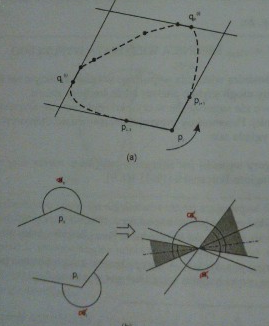
\includegraphics[width=0.3\textwidth]{img/diameter}
  \caption{Rysunek roboczy.\label{fig:diameter}}
\end{figure}

Wejściem dla algorytmu jest wielokąt zadany jako lista wierzchołków ze
wskaźnikiem na swój następnik w kolejności przeciwnej do ruchu
wskazówek zegara --- następnikiem wierzchołka $p_{n-1}$ jest
$p_0$. Dla czytelności algorytmu przyjmijmy także, że żadna para boków
tego wielokąta nie jest równoległa. Do określenia, który punkt leży
najdalej od odcinka $p_{i}p_{i+1}$, korzystamy z funkcji ,,podwojonego
pola ze znakiem trójkąta'' $p_{0}p_{i+1}p$, którą przedstawiono w
rozdziale~\ref{chap:pojecia} do wyznaczenia skrętności kąta. W
pierwszej części algorytmu w pętli \texttt{while} szukamy pierwszego
najdalszego wierzchołka i oznaczamy go jako $q_0$. Następnie
wyznaczamy łańcuch $C(p_i)$, używając wskaźników $p$ i $q$
poruszających się w kierunku odwrotnym do ruchu wskazówek zegara,
zaczynając odpowiednio od $p_0$ i $q_0$ do momentu, aż wskaźnik $q$
wróci do pozycji $p_0$. Po tym kroku zostaną wypisane wszystkie pary
antypodyczne. Znalezienie wierzchołka $q_0$ zajmuje w pesymistycznym
przypadku $N-1$ kroków, natomiast przejście po łańuchach $p_{0},
\ldots, q_{0}$ i $q_{0}, \ldots, p_{0}$ łącznie $N$ kroków. Mamy więc
do czynienia ze złożonością czasową rzędu $O(N)$.

% Specjalną sytuacją jest przypadek, gdy dwie krawędzie są równoległe
% (wtedy pole ze znakiem trójkąta jest równe dla dwóch wierzchołków
% tworzących krawędź równoległą), która wymaga od nas dodatkowego kroku
% przy każdym wierzchołku (wiersze 15--19).

% Poprawność algorytmu wynika z tego, że krawędzi równoległych jest co
% najwyżej $N/2$, więc łącznie algorytm nie wykonuje więcej niż $3N$
% kroków. Mamy więc do czynienia ze złożonością czasową rzędu $O(n)$.

Fakt, że punkt antypodyczny dla punktu $p_{i+1}$ nie może być bliższy
niż wierzchołek, który jest najdalej od $p_i$, wynika z wypukłością
wielokąta --- dla dowolnego wierzchołka $p$ można wyznaczyć taki
wierzchołek $q$, że odległość kolejnych wierzchołków od $p$ do $q$
jest nierosnąca, zaś od $q$ do $p$ --- niemalejąca.

\begin{figure}[htp]

  \begin{algorithmic}[1]
    \Procedure{Antipodal Pairs}{}

    \State $p \gets p_{n-1}$
    \State $q \gets NEXT[p]$

    \State

    \While {$NEXT[q]$ jest dalej od $(p, NEXT[p])$ niż $q$}
        \State {\emph{/* znajdźmy wierzchołek najdalszy od $(p, NEXT[p])$ */}}
        \State{$q \gets NEXT[p]$}

        \State

        \State {\emph{/* oznaczmy go jako $q_0$ */}}
        \State {$q_0 \gets q$}

        \State

        \While {$q \neq p_0$}
                \State {$p \gets NEXT[p]$}

                \State $print (p, q)$

                \State

                \While {$NEXT[q]$ jest dalej od odcinka $(p, NEXT[p])$ niż $q$}
                        \State $q \gets NEXT[q]$

                        \State

                        \State {\emph{/* jeżeli nie wróciliśmy do pozycji początkowej */ }}
                        \If {$(p, q) \neq (q_0,p_0)$}
                                \State $print (p, q)$
                        \EndIf
                \EndWhile
         \EndWhile
     \EndWhile
\EndProcedure

  \end{algorithmic}
  \caption{\label{alg:antipodal}}
\end{figure}

\begin{table}[htb]
  \centering

  \begin{tabular}{llll}
    \toprule
    $p$ & $q$ & para antypodyczna & krok \\
    \midrule
    $p_6$ & & & 1 \\
    \midrule
    & $p_0$ & & 3 \\
    \midrule
    & $p_1$ & & 5 \\
    \midrule
    & $p_2$ & & 5 \\
    \midrule
    & $p_3$ & & 5 \\
    \midrule
    $p_0$& & & 13 \\
    \midrule
    & & $(p_0, p_3)$ & 14 \\
    \midrule
    & $p_4$ & & 17 \\
    \midrule
    & & $(p_0, p_4)$ & 21 \\
    \midrule
    $p_1$& & & 13 \\
    \midrule
    & & $(p_1, p_4)$ & 14 \\
    \midrule
    & $p_5$ & & 17 \\
    \midrule
    & & $(p_1, p_5)$ & 21 \\
    \midrule
    $p_2$& & & 13 \\
    \midrule
    & & $(p_2, p_5)$ & 14 \\
    \midrule
    $p_3$& & & 13 \\
    \midrule
    & & $(p_3, p_5)$ & 14 \\
    \midrule
    & $p_6$ & & 17 \\
    \midrule
    & & $(p_3, p_6)$ & 21 \\
    \midrule
    & $p_0$ & & 17 \\
    \bottomrule
  \end{tabular}

  \caption{Ilustracja działania algorytmu  \textsc{Antipodal Pairs} dla
    wielokąta z rysunku~\ref{fig:antipodal}.}
\end{table}

%%% Local Variables:
%%% mode: latex
%%% TeX-master: "masterthesis"
%%% TeX-engine: xetex
%%% End:


% \section{Przecięcie wielokątów}
% \subsection{Shamos --- Hoey}
% \subsection{O'Rourke --- Nador}
% \subsection{Separating Axes}
% \section{Zawieranie wielokątów}
% \section{Wyznaczanie prostokąta zawierającego wielokąt}
% \section{Wyznaczanie największej odległości między wielokątami}
% \section{Złączanie wielokątów wypukłych}
% \section{Znajdowanie krytycznych linii wsparcia}
% \section{Oświetlenie wielokąta}

% \summary

% \appendix
% \chapter{Generowanie wielokątów wypukłych o zadanej liczbie
% wierzchołków}

% \bibliographystyle{unsrt}
% \bibliography{xml}

% \listoftables
% \listoffigures

% \oswiadczenie

\end{document}

%%% Local Variables:
%%% coding: utf-8
%%% mode: latex
%%% TeX-master: t
%%% TeX-engine: xetex
%%% End:
